\chapter{Wstęp}

\section{Używany sprzęt oraz narzędzia}

\begin{itemize}
    \item Stanowisko - \textbf{7}
    \item Oscyloskop - \textbf{MSO3012}
    \item Generator funkcyjny - \textbf{AFG3022B}
    \item Płytka - \textbf{W0-2}
    \item Multimetr - \textbf{2}
\end{itemize}

\section{Jednostki i przedrostki}

\begin{itemize}
    \item 1 Hz (herc) - jednostka miary częstotliwości - 1Hz = $\frac{1}{1s} = 1s^{-1}$
    \item 1 A (amper) - jednostka natężenia prądu elektrycznego - 1A = $\frac{1C}{1s}$
    \item 1 V (wolt) - jednostka potencjału elektrycznego, napięcia elektrycznego i siły elektromotorycznej - 1V = $\frac{1W}{1A}$ ($\frac{wat}{amper}$)
    \item 1 F (farad) - jednostka pojemności elektrycznej - 1F = $\frac{1C}{1V}$ ($\frac{kulomb}{wolt}$)
    \item 1 H (henr) - jednostka indukcyjności - 1H = $\frac{1 Wb}{1 A}$ ($\frac{weber}{amper})$
\end{itemize}

\begin{itemize}
    \item k (kilo) = $10^3$
    \item M (mega) = $10^6$
    \item m (mili) = $10^{-3}$
    \item $\mu$ (micro) = $10^{-6}$
    \item n (nano) = $10^{-9}$
\end{itemize}

\section{Wzmacniacz operacyjny i jego własności}
\label{sec:Wzmacniacz operacyjny}

\begin{itemize}
    \item Schemat wzmacniacza odwracającego fazę:
        \begin{figure}[H]
            \centering
            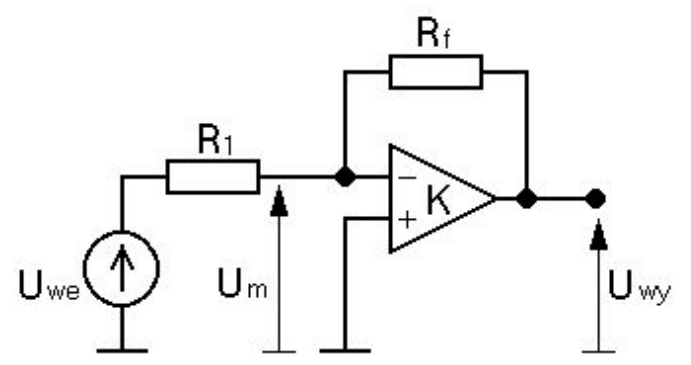
\includegraphics[scale=0.4]{img/schemes/wzmacniacz_operacyjny.png}
            \caption{Schemat wzmacniacza odwracającego fazę}
            \label{fig:schemat_wzmacniacz_odwracający}
        \end{figure}
    \item Wzór na napięcie wyjściowe:
        \begin{gather}
            \label{wzor:napiecie_wyjsciowe_odwracajacy}
            U_{wy} = -\dfrac{R_2}{R_1}U_{we}
        \end{gather}
    \item Schemat wzmacniacza nieodwracającego fazy:
        \begin{figure}[H]
            \centering
            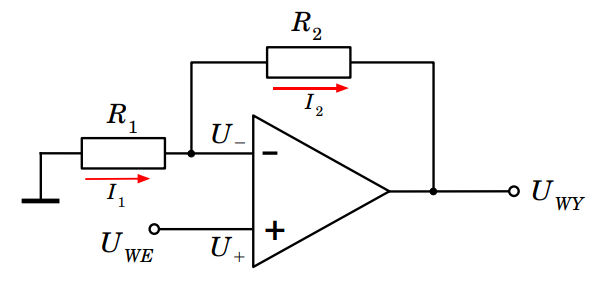
\includegraphics[scale=0.4]{img/schemes/wzmacniacz_operacyjny_nieodwracajacy.png}
            \caption{Schemat wzmacniacza nieodwracającego fazy}
            \label{fig:schemat_wzmacniacz_nieodwracający}
        \end{figure}
    \item Wzór na napięcie wyjściowe:
        \begin{gather}
            \label{wzor:napiecie_wyjsciowe_nieodwracajacy}
            U_{wy} = \dfrac{R_1 + R_2}{R_1}U_{we}
        \end{gather}
        
    \item Cechy idealnego wzmacniacza napięciowego:
        \begin{itemize}
            \item Nieskończenie duże wzmocnienie napięciowe: K $\xrightarrow{} \infty$
            \item Nieskończenie duża rezystancja wejściowa
            \item Rezystancja wyjściowa równa zeru
            \item Nieskończenie szerokie pasmo przenoszenia częstotliwości (od 0 do $\infty$)
            \item Napięcie wyjściowe równe zeru przy równych napięciach wejściowych
        \end{itemize}
\end{itemize}

\section{Wzmacniacz sumujący - sumator napięć}

\begin{itemize}
    \item Schemat sumatora:
        \begin{figure}[H]
            \centering
            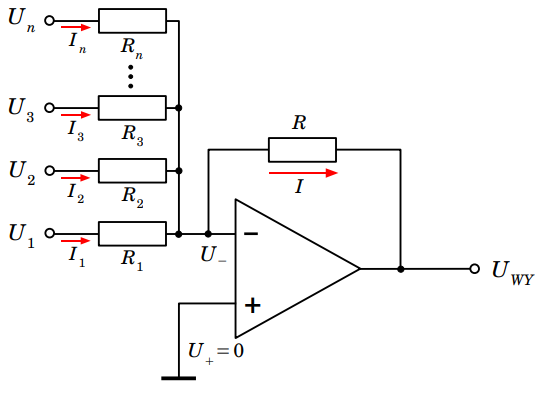
\includegraphics[scale=0.4]{img/schemes/sumator.png}
            \caption{Schemat sumatora}
            \label{fig:schemat_sumatora}
        \end{figure}
    \item Wzór na napięcie wyjściowe:
        \begin{gather}
            U_{wy} = -R(\dfrac{U_1}{R_1} + \dfrac{U_2}{R_2} + \dfrac{U_3}{R_3} + \dots + \dfrac{U_n}{R_n}) \\
            R_1 = R_2 = \dots = R \implies U_{wy} = -(U_1 + U_2 + \dots + U_n)
        \end{gather}
\end{itemize}

\section{Przerzutnik Schmidta}

\begin{itemize}
    \item Przerzutnik to układ elektroniczny wytwarzający prostokątne przebiegi napięciowe w wyniku szybkich procesów przełączania pomiędzy różnymi stanami.
    \item Przerzutnik Schmidta jest przerzutnikiem bistabilnym/dwustanowym. Dla wymuszenia przejścia z jednego stanu do drugiego konieczne jest doprowadzenie zewnętrznego sygnału wyzwalającego.
    \item Schemat przerzutnika:
        \begin{figure}[H]
            \centering
            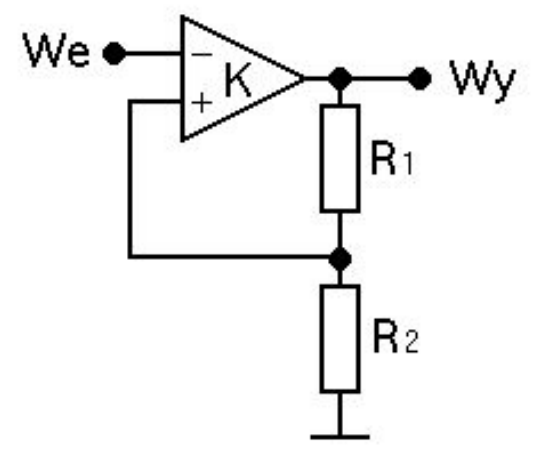
\includegraphics[scale=0.4]{img/schemes/przerzutnik_schmidta.png}
            \caption{Schemat przerzutnika}
            \label{fig:schemat_przerzutnika_schmidta}
        \end{figure}
\end{itemize}

\section{Multiwibrator astabilny}

\begin{itemize}
    \item Okres drgań układu:
        \begin{align}
            \label{eq:multiwibrator_okres_drgań} T = 2RC\ln({\dfrac{1+\gamma}{1-\gamma}}) \\
            \label{eq:multiwibrator_gamma} \gamma = \dfrac{R_2}{R_1+R_2}
        \end{align}
    \item Schemat multiwibratora astabilnego:
        \begin{figure}[H]
            \centering
            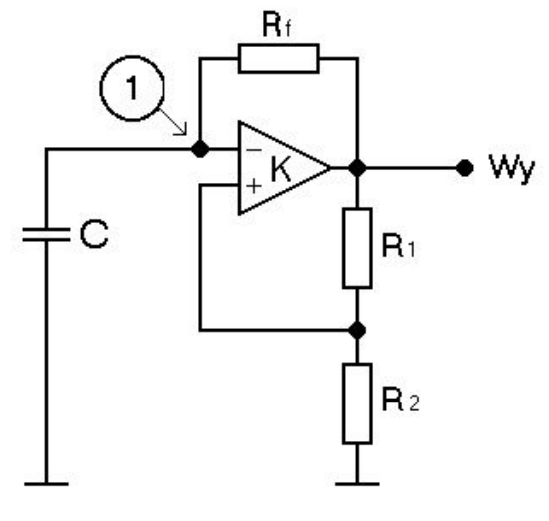
\includegraphics[scale=0.4]{img/schemes/multiwibrator.png}
            \caption{Schemat multiwibratora astabilnego}
            \label{fig:schemat_multiwibratora}
        \end{figure}
\end{itemize}